
\documentclass[letterpaper, reqno,11pt]{article}
\usepackage[margin=1.0in]{geometry}
\usepackage{color,latexsym,amsmath,amssymb}
\usepackage{fancyhdr}
\usepackage{amsthm}
\usepackage[linesnumbered,lined,boxed,commentsnumbered,noend,noline]{algorithm2e}
\usepackage{dsfont}
\usepackage{graphicx}
\usepackage{hyperref}
\usepackage{bbm}
\usepackage[inline]{enumitem}
\usepackage[numbers]{natbib}
\usepackage{framed}
\usepackage{titling}
\usepackage{subcaption}
\usepackage[dvipsnames]{xcolor}
\usepackage{tikz}

\tikzset{invclip/.style={clip,insert path={{[reset cm]
  (-16383.99999pt,-16383.99999pt) rectangle (16383.99999pt,16383.99999pt)}}}}

\allowdisplaybreaks

\newcommand{\RR}{\mathbb{R}}
\newcommand{\CC}{\mathbb{C}}
\newcommand{\ZZ}{\mathbb{Z}}
\newcommand{\QQ}{\mathbb{Q}}
\newcommand{\NN}{\mathbb{N}}
\newcommand{\FF}{\mathbb{F}}
\newcommand{\PP}{\mathbb{P}}
\newcommand{\EE}{\mathbb{E}}
\newcommand{\LL}{\mathbb{L}}
\newcommand{\TT}{\mathbb{T}}
\DeclareMathOperator{\conv}{conv}
\DeclareMathOperator{\charcone}{char.cone}
\DeclareMathOperator{\STAB}{STAB}
\DeclareMathOperator{\Down}{Down}
\DeclareMathOperator{\lca}{lca}
\DeclareMathOperator{\ex}{ex}
\DeclareMathOperator{\Span}{span}
\DeclareMathOperator{\T}{T}
\DeclareMathOperator{\F}{F}
\DeclareMathOperator{\shP}{\# P}
\DeclareMathOperator{\shSAT}{\# SAT}
\DeclareMathOperator{\shDNF}{\# DNF}
\DeclareMathOperator{\DNF}{DNF}
\DeclareMathOperator{\Poly}{P}
\DeclareMathOperator{\CNF}{CNF}
\DeclareMathOperator{\SAT}{SAT}
\DeclareMathOperator{\BPP}{BPP}
\DeclareMathOperator{\poly}{poly}
\newcommand\mycommfont[1]{\ttfamily\textcolor{blue}{#1}}
\SetCommentSty{mycommfont}
\begin{document}
\pagenumbering{arabic}
\title{Lectures on Uniform Generation and Approximate Counting}
\author{Yuchong Pan}
\date{\today}
\newtheorem{theorem}{Theorem}
\newtheorem{lemma}[theorem]{Lemma}
\newtheorem{proposition}[theorem]{Proposition}
\newtheorem{corollary}[theorem]{Corollary}
\newtheorem{fact}[theorem]{Fact}
\newtheorem{claim}{Claim}
\newtheorem{exercise}{Exercise}
\theoremstyle{definition}
\newtheorem{definition}[theorem]{Definition}
%\maketitle
%

\begin{framed}
\noindent{\bf 6.842 Randomness and Computation} \hfill \thedate
\begin{center}
\Large{\thetitle}
\end{center}
\noindent{\em Lecturer: Ronitt Rubinfield} \hfill {\em Scribe: \theauthor}
\end{framed}

\section{Uniform Generation for DNF}

A \emph{DNF formula} is a Boolean formula that consists of ``OR of ANDs'', e.g., $\varphi(x_1, x_2, x_3) = x_1 \overline{x_2} \vee \overline{x_1} x_3$. The task is to output a random satisfying assignment to a DNF formula, uniformly over all satisfying assignments.

Consider the special case with only one conjunction. We can satisfy literals in the conjunction, and set the others randomly. For instance, for $\varphi(x_1, x_2, x_3) = x_1 \overline{x_2}$, we set $x_1 = \T, x_2 = \F$, and set $x_3 \in \{ \T, \F \}$ uniformly.

Now consider the two conjunction case, e.g., $\varphi(x_1, x_2, x_3) = x_1 x_2 \vee x_3$. We give an algorithm attempt in Algorithm \ref{alg:2-conj}. However, two problems arise, as illustrated in Figure \ref{fig:2-conj}. Firstly, conjunctions have different numbers of assignments. Secondly, some assignments can be chosen in multiple ways. In particular, using Algorithm \ref{alg:2-conj}, the probability that TTF is chosen is $1/2 \cdot 1/2 = 1/4$, the probability that TTT is chosen is $1/2 \cdot 1/2 + 1/2 \cdot 1/4 = 3/8$, and that the probability that each of TFT, FTT, FFT is chosen is $1/2 \cdot 1/4 = 1/8$.

\begin{algorithm}
  pick $i \in \{ 1, 2 \}$ uniformly \\
  set variables in conjunction $i$ to T \label{line:conj} \\
  set others uniformly
  \caption{An algorithm attempt of uniform generation for DNF with 2 conjunctions.}
  \label{alg:2-conj}
\end{algorithm}

\begin{figure}[h]
  \centering
  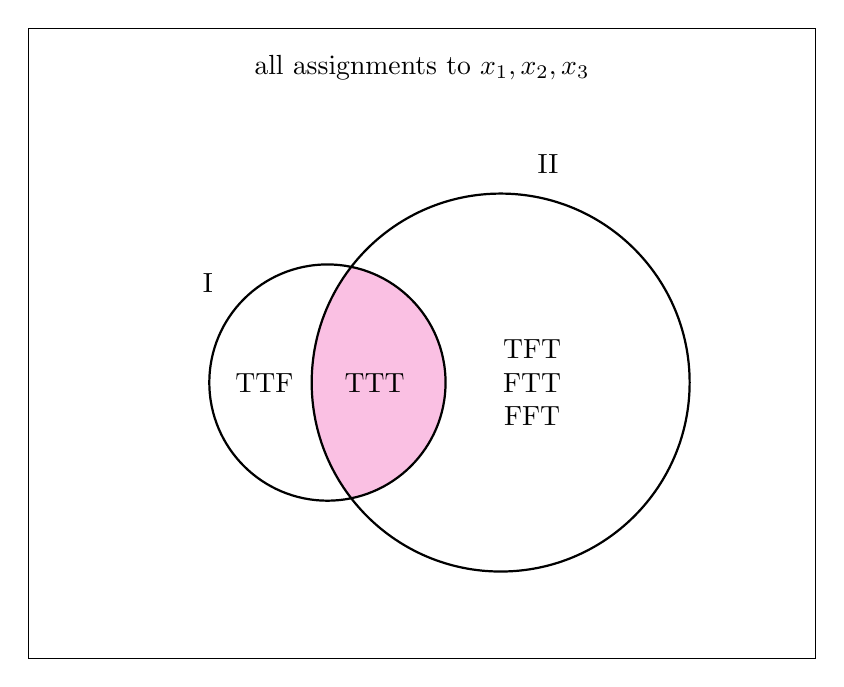
\begin{tikzpicture}
    \def\firstcircle{(180:1.2) circle[radius = 1.5]}
    \def\secondcircle{(0:1) circle[radius = 2.4]}

    \node at (155:3) {I};
    \node at (60:3.2) {II};

    \begin{scope}
      \clip \firstcircle;
      \fill[fill=Rhodamine!30] \secondcircle;
    \end{scope}
    \draw[thick] \firstcircle \secondcircle;

    \node at (180:2) {TTF};
    \node at (180:.6) {TTT};
    \node[align=center] at (0:1.4) {TFT \\ FTT \\ FFT};

    \draw (-5, 4.5) rectangle (5, -3.5);

    \node at (0, 4) {all assignments to $x_1, x_2, x_3$};
  \end{tikzpicture}
  \caption{An illustration of problems in Algorithm \ref{alg:2-conj}.}
  \label{fig:2-conj}
\end{figure}

The first problem is easy to fix; we simply replace line \ref{line:conj} in Algorithm \ref{alg:2-conj} to ``pick $i \in \{ 1, 2 \}$ \emph{proportional to the number of satisfying assignments for that conjunction}.'' For the second problem, we introduce the notion of \emph{rejection sampling}. Let $m$ be the number of conjunctions in $\varphi$. For each $i \in [m]$, let $A_i = \{ \bar x = (x_1, \ldots, x_n) : \text{$\bar x$ satisfies the $i^\text{th}$ conjunction} \}$. Consider the example illustrated in Figure \ref{fig:rej-samp}. In the shaded region in Figure \ref{fig:rej-samp}, each assignment is $3$ times more likely to be picked; therefore, we correct our algorithm by tossing a coin of bias $1/3$ to decide if to output the assignment. We summarize our final algorithm in Algorithm \ref{alg:unif-gen}.

\begin{figure}
  \centering
  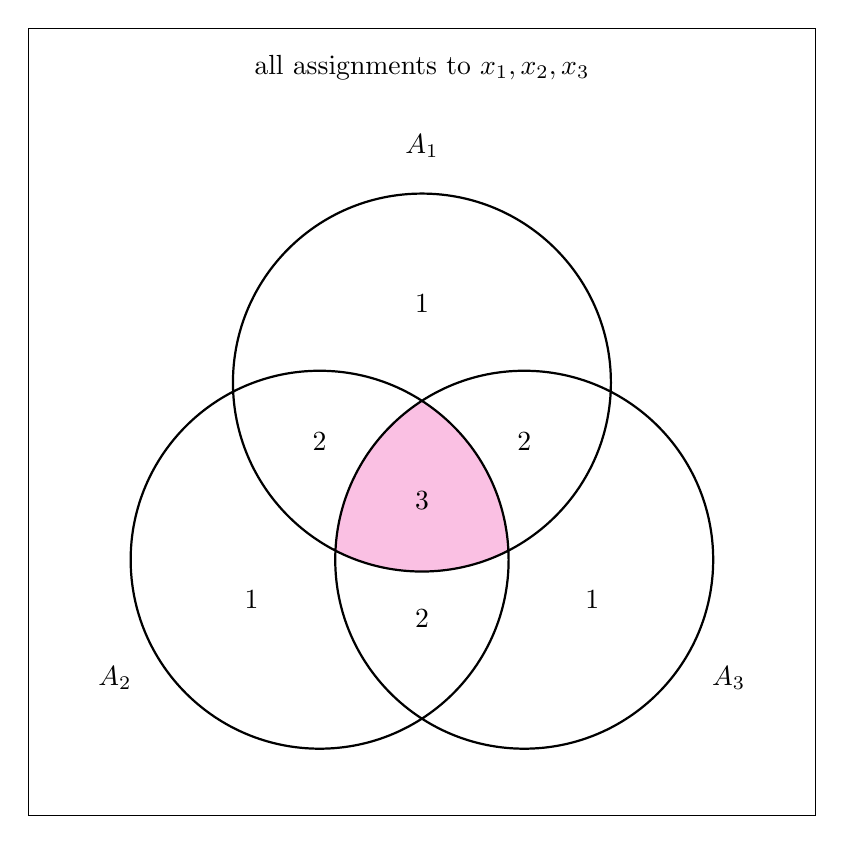
\begin{tikzpicture}
    \def\firstcircle{(90:1.5) circle[radius = 2.4]}
    \def\secondcircle{(210:1.5) circle[radius = 2.4]}
    \def\thirdcircle{(330:1.5) circle[radius = 2.4]}

    \node at (90:4.5) {$A_1$};
    \node at (210:4.5) {$A_2$};
    \node at (330:4.5) {$A_3$};

    \begin{scope}
      \clip \firstcircle;
      \clip \secondcircle;
      \fill[fill=Rhodamine!30] \thirdcircle;
    \end{scope}
    \draw[thick] \firstcircle \secondcircle \thirdcircle;

    \node at (270:1.5) {$2$};
    \node at (0:0) {$3$};
    \node at (150:1.5) {$2$};
    \node at (30:1.5) {$2$};
    \node at (90:2.5) {$1$};
    \node at (210:2.5) {$1$};
    \node at (330:2.5) {$1$};

    \draw (-5, 6) rectangle (5, -4);

    \node at (0, 5.5) {all assignments to $x_1, x_2, x_3$};
  \end{tikzpicture}
  \caption{An example for rejection sampling, where the number in each region indicates the number of conjunctions each assignment satisfies.}
  \label{fig:rej-samp}
\end{figure}

\begin{algorithm}
  \DontPrintSemicolon
  $A_i = \{ \bar x = (x_1, \ldots, x_n) : \text{$\bar x$ satisfies the $i^\text{th}$ conjunction} \}$ for each $i \in [m]$ \\
  \Repeat{success}{
    pick $i \in [m]$ with probability $|A_i|/\sum_{j = 1}^m |A_j|$ \\
    pick $\bar b \in A_i$ uniformly \\
    $t_{\bar b} \leftarrow |\{ j \in [m] : \bar b \in A_j \}|$ \CommentSty{// $t_{\bar b} \geq1$ since $\bar b$ satisfies $C_i$} \\
    output $\bar b$ with probability $1/t_{\bar b}$
  }
  \caption{Uniform generation for DNF, where the input is a DNF formula $\varphi = \bigvee_{i = 1}^m C_i$ and $C_i$ is a conjunction for each $i \in [m]$.}
  \label{alg:unif-gen}
\end{algorithm}

We show the uniformity of Algorithm \ref{alg:unif-gen}. For each $\bar b$ that satisfies $\varphi$,
\begin{align*}
  \PP\left[\text{$\bar b$ is output in round $i$}\right] &= \frac{1}{t_{\bar b}} \sum_{\substack{j \in [m] \\ \bar b \in A_j}} \PP[\text{pick $j$ in round $i$}] \cdot \frac{1}{\left|A_j\right|} \\
  &= \frac{1}{t_{\bar b}} \sum_{\substack{j \in [m] \\ \bar b \in A_j}} \frac{\left|A_j\right|}{\sum_{k = 1}^m \left|A_k\right|} \cdot \frac{1}{\left|A_j\right|} \\
  &= \frac{1}{t_{\bar b}} \sum_{\substack{j \in [m] \\ \bar b \in A_j}} \frac{1}{\sum_{k = 1}^m \left|A_k\right|} \\
  &= \frac{1}{\sum_{k = 1}^m \left|A_k\right|}.
\end{align*}
Hence, the probability that $\bar b$ is output in round $i$ is the same for all $\bar b$ satisfying $\varphi$, so the generation is uniform. Moreover, $\PP[\text{loop success}] \geq 1/\max t_{\bar b}\geq 1/m$, so $\EE[\text{\# loops until success}] \leq m$. This shows that Algorithm \ref{alg:unif-gen} runs in polynomial time in expectation.

\section{Counting Problems}

\begin{definition}
  Let $\shP$ denote the class of problems that count the number of accepting paths in a polynomial time nondeterministic Turing machines.
\end{definition}

\begin{definition}
  We say that a problem is \emph{$\shP$-complete} if
  \begin{enumerate}[label=(\alph*), itemsep=0pt]
    \item it is in $\shP$;
    \item every problem in $\shP$ has a polynomial time reduction to it.
  \end{enumerate}
\end{definition}

Let $\shSAT$ denote the problem that counts the number of assignments satisfying a Boolean formula $\varphi$. Then $\shSAT$ is $\shP$-complete. Similarly, let $\shDNF$ denote the problem that counts the number of assignments satisfying a DNF formula $\varphi$. Although $\DNF \in \Poly$, we show below that $\shDNF \not \in \Poly$. However, it turns out that $\shDNF$ is $\shP$-complete.

\begin{proposition}
  $\shDNF \not \in \Poly$.
\end{proposition}

\begin{proof}
  We show that if $\shDNF \in \Poly$, then $\CNF \in \Poly$. By De Morgan's law, a clause $\overline{A \vee B} = \overline{A} \wedge \overline{B}$, which is a conjunction. Therefore, Given a CNF formula $\varphi$ in $n$ variables, $\varphi$ is satisfiable if and only if $\overline \varphi$ (which is a DNF formula) has at most $2^n - 1$ satisfying assignments.
\end{proof}

\section{Approximate Counting and Downward Self-Reducibility} \label{sec:approx-counting}

\begin{definition} \label{def:fpras}
  A \emph{fully polynomial randomized approximation scheme (FPRAS)} for DNF is an algorithm which, given a DNF formula $\varphi$ and $\varepsilon > 0$, outputs $y \in \ZZ_+$ such that $z/(1 + \varepsilon) \leq y \leq z(1 + \varepsilon)$ with probability at least $3/4$ in time polynomial in $|\varphi$ and $1/\varepsilon$, where $z$ is the number of satisfying assignments to $\varphi$.
\end{definition}

In Problem Set 1 Problem 1, we shall show that Definition \ref{def:fpras} implies that an FPRAS runs in time polynomial in $|\varphi|$, $1/\varepsilon$ and $\log \delta$ if we replace the probability bound $3/4$ with $1 - \delta$.

\begin{proposition}
  If there exists an FPRAS for $\shSAT$, then $\SAT \in \BPP$.
\end{proposition}

\begin{proof}
  We give a probabilistic algorithm for SAT. Given a Boolean formula $\varphi$, we call the FPRAS on $\varphi$ with $\varepsilon = 1/2$ (or any constant); if the output of the FPRAS is positive, then output ``satisfiable''; else output ``unsatisfiable.''

  If $\varphi$ is satisfiable, then the number of satisfying assignments is at least $1$, so $y \geq 1/(1 + \varepsilon) > 0$, which impies that the algorithm outputs ``satisfiable.'' Otherwise, the number of satisfying assignments is $0$, so $y = 0$, which implies that the algorithm outputs ``unsatisfiable.''
\end{proof}

\emph{Downward self-reducibility (DSR)} refers to the idea of solving a problem via solving its sub-problems. For DNF, we can compute the number of satisfying assignments using the DSR tree in Figure \ref{fig:dsr}, where $F_{b_1, \ldots, b_k}$ denotes the number of satisfying assignments for $\varphi(b_1, \ldots, b_k, x_{k + 1}, \ldots, x_n)$.

\begin{figure}[h]
  \centering
  \begin{tikzpicture}
    \fill[black] (0, 0) circle (2pt) node[above, yshift=10pt] (f) {$F = \# \varphi(x_1, \ldots, x_n)$};
    \fill[black] (-2, -1) circle (2pt) node[left, xshift=-10pt] (f0) {$F_0 = \# \varphi(0, x_2, \ldots, x_n)$};
    \fill[black] (2, -1) circle (2pt) node[right, xshift=10pt] (f1) {$F_1 = \# \varphi(1, x_2, \ldots, x_n)$};
    \fill[black] (-3, -2) circle (2pt) node[left] (f00) {};
    \fill[black] (-1, -2) circle (2pt) node[left] (f01) {};
    \fill[black] (1, -2) circle (2pt) node[left] (f10) {};
    \fill[black] (3, -2) circle (2pt) node[right, xshift=10pt] (f11) {$F_{11} = \# \varphi(1, 1, x_3, \ldots, x_n)$};

    \draw (0, 0) -- (-2, -1);
    \draw (0, 0) -- (2, -1);
    \draw (-2, -1) -- (-3, -2);
    \draw (-2, -1) -- (-1, -2);
    \draw (2, -1) -- (1, -2);
    \draw (2, -1) -- (3, -2);

    \node at (0, -2.5) {$\vdots$};
    
    \fill[black] (-3.5, -3.5) circle (2pt);
    \fill[black] (-2.5, -3.5) circle (2pt);
    \fill[black] (-1.5, -3.5) circle (2pt);
    \fill[black] (-0.5, -3.5) circle (2pt);
    \fill[black] (0.5, -3.5) circle (2pt);
    \fill[black] (1.5, -3.5) circle (2pt);
    \fill[black] (2.5, -3.5) circle (2pt);
    \fill[black] (3.5, -3.5) circle (2pt) node[right, xshift=10pt] {$F_{b_1, \ldots, b_n} = \# \varphi(b_1, \ldots, b_n) \in \{ 0, 1 \}$};
  \end{tikzpicture}
  \caption{The DSR tree for DNF.}
  \label{fig:dsr}
\end{figure}

WLOG consider the root of the DSR tree. Then $F = F_0 + F_1$. Let $S_1 = F_1/F$ be the fraction of satisfying assignments for which $x_1 = \T$. Then $F = F_1/S_1$, where $F_1$ can be computed recursively via $F_1 = F_{11}/S_{11}$, with $S_{11}$ the fraction of satisfying assignments to $\varphi(1, x_2, \ldots, x_n)$ for which $x_2 = \T$. The main insights of approximate counting for DNF are:
\begin{enumerate}[label=(\roman*), itemsep=0pt]
  \item we can estimate $S_1$ via sampling;
  \item we can uniformly generate satisfying assignments for DNF.
\end{enumerate}
To estimate $S_1$, we use the simple algorithm in Algorithm \ref{alg:est}.

\begin{algorithm}
  uniformly generate $k$ satisfying assignments to $\varphi$ \\
  $\widetilde{S_1} \leftarrow (\text{\# generated satisfying assignments with $x_1 = \T$})/k$
  \caption{An algorithm that estimates $S_1$.}
  \label{alg:est}
\end{algorithm}

For $k \in \ZZ_+$ and $b_1, \ldots, b_k \in \{ 0, 1 \}$, define $S_{b_1, \ldots, b_n}$ to be the fraction of satisfying assignments to $\varphi(b_1, \ldots, b_{k - 1}, x_k, \ldots, x_n)$ for which $x_k = b_k$ (note that we use T/F and $1$/$0$ interchangeably), and $\widetilde{S_{b_1, \ldots, b_k}}$ to be the estimate of $S_{b_1, \ldots, b_k}$ similarly computed as in Algorithm \ref{alg:est}. For $b_1, \ldots, b_n \in \{ 0, 1 \}$,
$$ F = \frac{F_{b_1}}{S_{b_1}} = \frac{1}{S_{b_1}} \cdot \frac{F_{b_1, b_2}}{S_{b_1, b_2}} = \frac{F_{b_1, b_2, b_3}}{S_{b_1} S_{b_1, b_2} S_{b_1, b_2, b_3}} = \ldots = \frac{1}{\prod_{i = 1}^n S_{b_1, \ldots, b_i}}. $$

Two difficulties arise:
\begin{enumerate}[label=(\roman*), itemsep=0pt]
  \item What if $F_{b_1, \ldots, b_i} = 0$ for some $i \in [n]$?
  \item Are the approximations of $S_{b_1, \ldots, b_i}$'s for $i \in [n]$ enough?
\end{enumerate}
The solution to both of the difficulties are to always go down to the ``large enough'' child. We note that for the choice of the ``larger'' child, a small additive error implies a small multiplicative error. To see this, suppose that we estimate each $S_{b_1, \ldots, b_i}$ to within an additive error of $\varepsilon/(18n)$ (by Chernoff's bound, we need $\poly(n/\varepsilon)$ samples). Therefore, if $1/3 \leq r \leq 1$, then
\begin{align*}
  r + \frac{\varepsilon}{18n} &= r\left(1 + \frac{\varepsilon}{18nr}\right) \leq r\left(1 + \frac{\varepsilon}{6n}\right), \\
  r - \frac{\varepsilon}{18n} &= r\left(1 - \frac{\varepsilon}{18nr}\right) \geq r\left(1 - \frac{\varepsilon}{6n}\right).
\end{align*}
Therefore, the output is at most
$$ \frac{F_{b_1}}{\widetilde{S_{b_1}}} \leq \ldots \leq \frac{1}{\prod_{i = 1}^n \widetilde{S_{b_1, \ldots, b_i}}} \leq \frac{1}{\prod_{i = 1}^n S_{b_1, \ldots, b_n} \left(1 - \frac{\varphi}{6n}\right)} \leq \frac{\left(1 + \frac{\varepsilon}{3n}\right)^n}{\prod_{i = 1}^n S_{b_1, \ldots, b_n}} \leq F\left(1 + \frac{\varepsilon}{2}\right). $$
We can similarly show that the output is at least $F/(1 + \varepsilon)$.

\section{Equivalence Between Uniform Generation and Counting}

\begin{theorem}[Jerrum-Valiant-Vazirani]
  For any problem in NP that is downward self-reducible, one can approximately count the number of solutions to the problem in polynomial time if and only if one can perform generate solutions to the problem almost uniformly in polynomial time.
\end{theorem}

In this note, we prove the easier case where both of uniform generation and counting are perfect. That perfect uniform generation implies perfect counting is proved in Section \ref{sec:approx-counting}. For the other direction, given a counter for $\shDNF$, we define a recursive algorithm in Algorithm \ref{alg:counter-implies-unifgen} that performs uniform generation for DNF. For any satisfying assignment $b_1, \ldots, b_n$, the probability that Algorithm \ref{alg:counter-implies-unifgen} outputs $b_1, \ldots, b_n$ is
$$ \frac{F_{b_1}}{F} \cdot \frac{F_{b_1, b_2}}{F_{b_1}} \cdots \frac{1}{F_{b_1, \ldots, b_{n - 1}}} = \frac{1}{F}. $$
Therefore, the probability that every satisfying assignment is output by Algorithm \ref{alg:counter-implies-unifgen} is equal, so Algorithm \ref{alg:counter-implies-unifgen} is a uniform generator for DNF.

\begin{algorithm}
  \CommentSty{// at $b_1, \ldots, b_i$} \\
  use the counter to compute $r_0 = F_{b_1, \ldots, b_i, 0}$ and $r_1 = F_{b_1, \ldots, b_i, 1}$ \\
  go left on the DSR tree with probability $r_0/(r_0 + r_1)$; else go right \\
  output $b_1, \ldots, b_n$ when reaching a leaf
  \caption{A uniform generator for DNF given a counter.}
  \label{alg:counter-implies-unifgen}
\end{algorithm}

\end{document}
